\newpage
\section{Auswertung}

\subsection{Entladevorgange des Kondensators}
\label{sub:a}
    Durch die Beobachtung des Entladevorganges des Kondensators kann die Zeitkonstante des RC-Glieds bestimmt werden. Durch Messungen am Oszilloskop folgen folgende Werte:
        \begin{table}
        \centering
        \begin{tabular}{c c}
            \toprule
            {Spannung U in $\si{\volt}$} & {Zeit t in $\si{\micro\second} $} \\
            \midrule
            -2.30 & 30    \\
            -3.14 & 0     \\
            -2.64 & -220  \\
            -2.00 & -440  \\
            -1.20 & -720  \\
            -0.40 & -900  \\
                0 & -1000 \\
            0.400 & -1075 \\
            0.880 & -1160 \\
             1.25 & -1215 \\
             1.92 & -1330 \\
             2.56 & -1410 \\
             3.36 & -1510 \\
             3.94 & -1570 \\
             4.48 & -1630 \\
             4.6  & -1650 \\ 
             4.32 & -1790 \\
             4.48 & -1730 \\
            \bottomrule
        \end{tabular}
        \caption{Messdaten zur Entladung}
        \label{tab:a}
        \end{table}

    \noindent
    Diese Daten werden nun geplottet und eine Ausgleichsfunktion wird durchgelegt. Die Ausgleichsfunktion ergibt sich aus der Gleichung (\ref{eqn:e}) und der Formel $ Q = CU $ zu 
    
    \begin{equation}
    U(t) = U_0 \,  \exp\left(-\frac{t}{\symup{RC}}\right)
    \end{equation}

    \noindent
    Um die Grafik optisch schöner zu skalieren wird derZeitpunkt $t=0$ auf den höchst gemessenen Spannungspunkt gelegt. Zudem wird der Graph halblogaritmisch abgebildet. Daraus folgt dann
    folgende Grafik.

    \begin{figure}
        \centering
        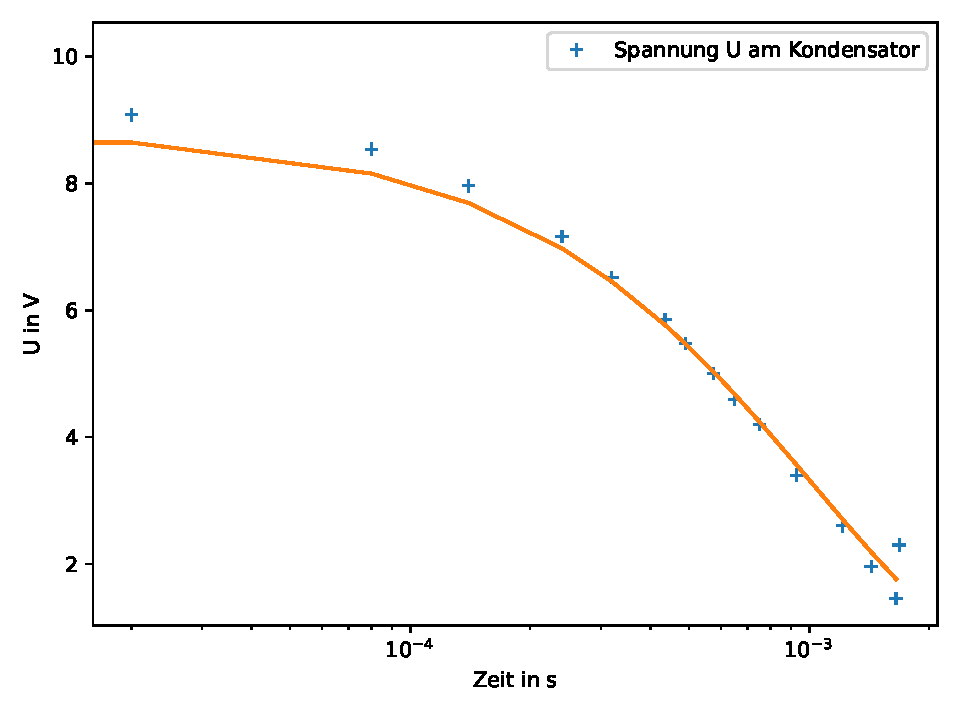
\includegraphics[width=\textwidth]{Daten/a.pdf}
        \caption{$U_\text{C} \, / \, \si{\volt}$ gegen die Zeit $t$ aufgetragen.}
    \end{figure}

    \noindent
    Aus der Ausgleichsgerade folgt $U_0 = 8.8156 \pm 0.1659 \si{\volt}$ und $RC = 0.0010262 \pm 0.0000517 \si{\second} $.
\newpage
\subsection{Amplitude und Frequenz}
    Als nächstes wird die doppelte Amplitude $U_\text{C}$ in der Abhängigkeit der Frequenz betrachtet. Diese gemessen ergeben dann folgende Messwerte:
    \begin{table}
        \centering
        \begin{tabular}{c c}
            \toprule
            {Frequenz f in $\si{\hertz}$} & {doppelte Spannung $U_\text{C}$ in $\si{\volt}$} \\
            \midrule
            10   & 12.16 \\
            20   & 11.92 \\
            30   & 11.52 \\
            40   & 11.36 \\
            50   & 11.20 \\
            100  &  9.52 \\
            200  &  6.88 \\
            300  &  5.12 \\
            400  &  4.12 \\
            500  &  3.36 \\
            1000 &  1.82 \\          
            2000 & 0.952 \\
            3000 & 0.628 \\
            4000 & 0.488 \\
            5000 & 0.380 \\
            \bottomrule
        \end{tabular}
    \caption{Messdaten zur Entladung}
    \label{tab:b}
    \end{table}

    \noindent
    Zusätzlich wird $U_0 = 6.88V$ gemessen. Die gemessenen Werte werden als ebenfalls in ein halblogarithmischen Diagramm, sowie in (\ref{sub:a}), aufgetragen und eine Ausgleichsfunktion nach Gleichung (\ref{eqn:sqrt}) der Form
    
    \begin{equation}
        \frac{A(\omega)}{U_0} = \frac{1}{\sqrt{1+\omega^2R^2C^2}} = \frac{1}{\sqrt{1+(2 \pi f)^2R^2C^2}}
    \end{equation}

    \noindent
    wird durchgelegt.
    \begin{figure}
        \centering
        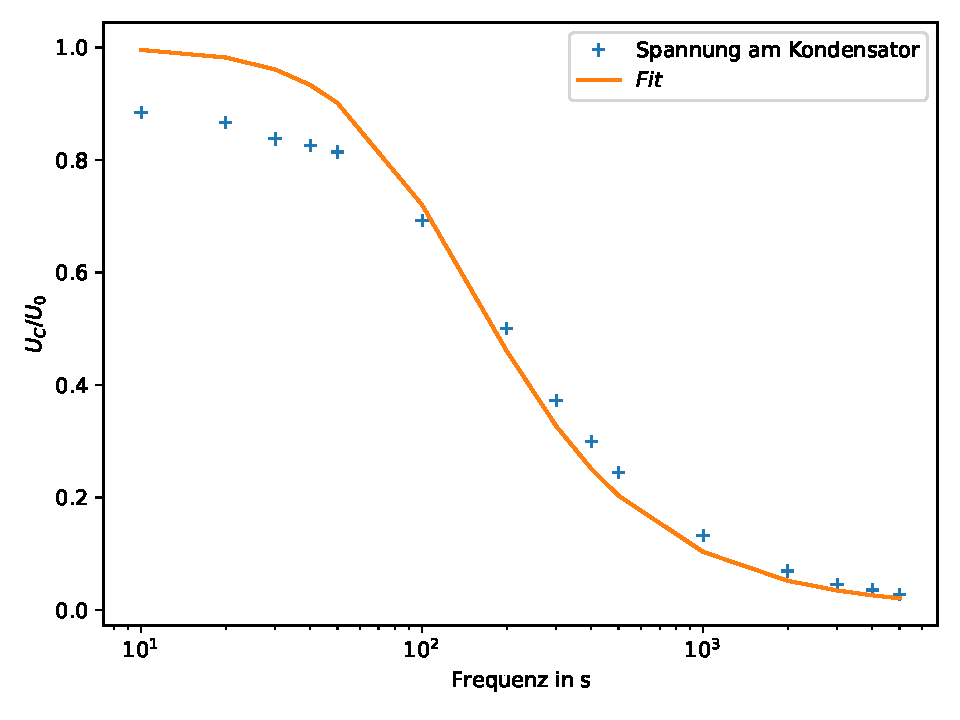
\includegraphics[width=\textwidth]{Daten/b.pdf}
        \caption{$\frac{A(\omega)}{U_0}$ gegen die Frequenz $f$ aufgetragen.}
    \end{figure}

    \noindent
    Die Ausgleichfunktion liefert für $RC = 0.00153 \pm 0.00015 \si{\second}$.
\newpage
    \subsection{Phasenverschiebung}
    Die Phasenverschiebung wird nach Abbildung (6) ermittelt. Als Tabelle aufgetragen folgen folgende Messwerte:
\begin{table}
        \centering
        \begin{tabular}{c c c}
            \toprule
            {Frequenz f in $\si{\hertz}$} & {a in $\si{\micro\second}$} & {b in $\si{\micro\second}$}\\
            \midrule
            10   & 5600 & 100000 \\
            20   & 1200 &  50000 \\
            30   & 1200 &  33000 \\
            40   &  800 &  25000 \\
            50   & 1000 &  20200 \\
            100  & 1000 &  10000 \\
            200  &  720 &   5000 \\
            300  &  600 &   3400 \\
            400  &  440 &   2480 \\
            500  &  360 &   2000 \\
            1000 &  220 &   1000 \\
            2000 &  112 &    500 \\
            3000 &   76 &    336 \\
            4000 &   60 &    250 \\
            5000 &   50 &    198 \\
            \bottomrule
        \end{tabular}
    \caption{Messdaten zur Phasenverschiebung}
    \label{tab:c}
    \end{table}

\noindent
    Nun werden die Daten in ein Diagramm aufgetragen und $\varphi$ nach 
    \begin{equation}
	\varphi = \frac{a}{b} \cdot 2\pi
	\label{eqn:4b-phase}
    \end{equation}
    berechnet. Die ermittelten Werte werden nun in ein f-$\varphi$-Diagramm geplotet und wie im Kapitel davor ausgewertet.

    \begin{figure}
        \centering
        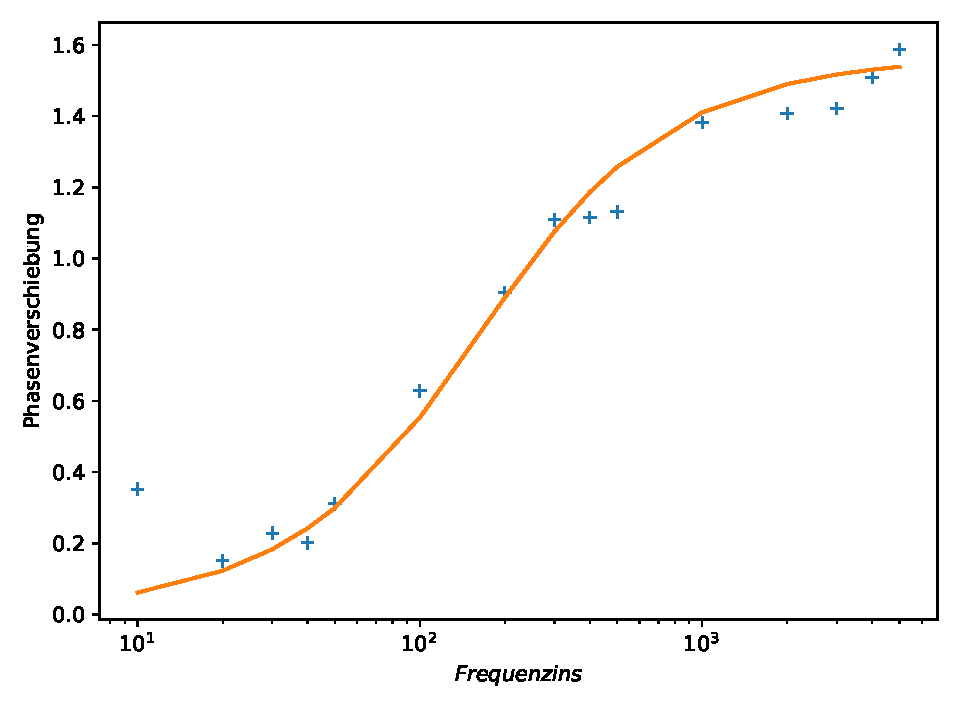
\includegraphics[width=\textwidth]{Daten/c.pdf}
        \caption{$f \, / \, \si{\hertz}$ gegen die Phasenverschiebung $\varphi$ aufgetragen.}
    \end{figure}
    
    Aus der Ausgleichfunktion ist gegeben durch (\ref{eqn:phi}). Aus dieser folgt für $RC = 0.0009829 \pm 0.00095 \si{\second}$.

    Zusätzlich kann mit den Werten aus der Tabelle (\ref{tab:b}) und dem zuvor ermittelten Wert für $RC$ die Werte in einem Polarkoordinatensystem dargestellt werden. Dieser sieht wie folgt aus:

    \begin{figure}
        \centering
        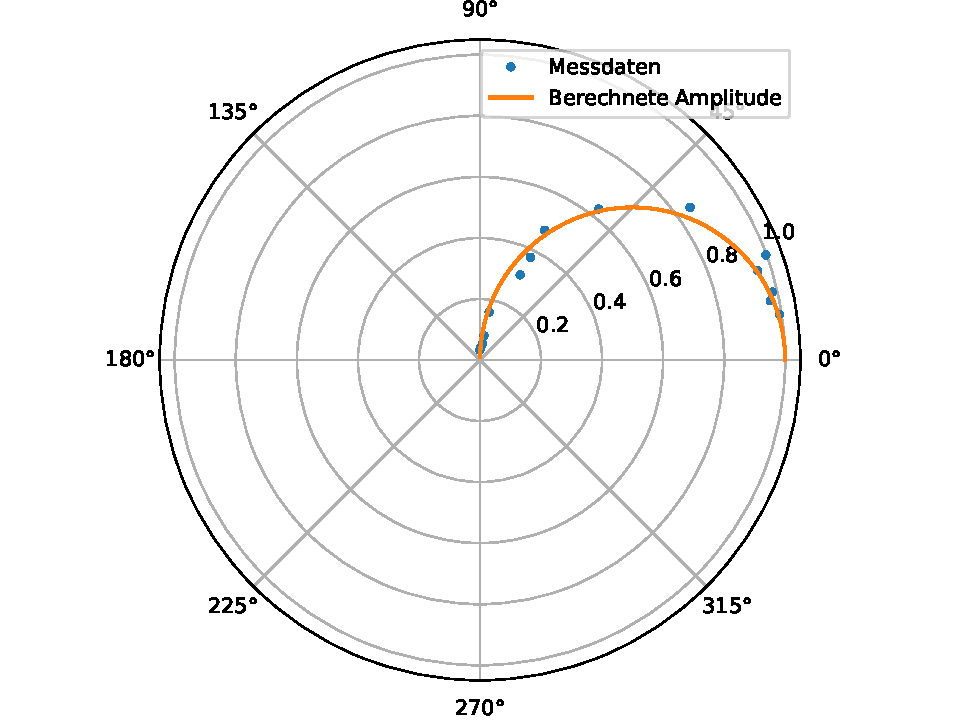
\includegraphics[width=\textwidth]{Daten/d.pdf}
        \caption{Radial wird das Amplitudenverhältnis, im Polarwinkel die Phasenverschiebung dargestellt.}
    \end{figure}
\newpage
\subsection{Integrator-Funktion des RC-Kreises}
    Der RC Kreis kann unter bestimmten Voraussetzungen als Integrator arbeiten. Die Integrationsfunktion ist dann gegeben durch die Formel (\ref{eqn:int}). In den folgenden Bildern vom
    Bildschirm des Oszilators ist oben die angelegte Spannung und unten die Kondensatorspannung dargestellt.

    \begin{figure}[H]
	\centering
	\begin{subfigure}[b]{0.3\textwidth}
		\centering
		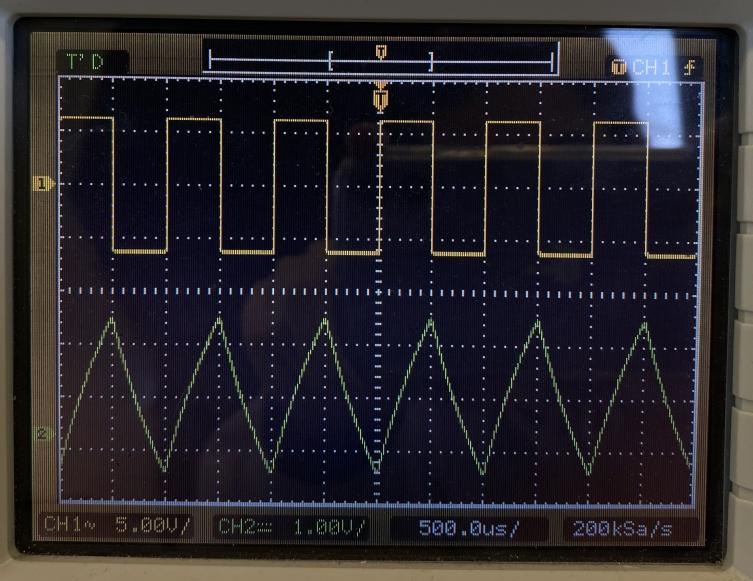
\includegraphics[width=4.5cm]{Rechteck.jpg}
		\caption{Rechtecksspannung}
	\end{subfigure}
	~
	\begin{subfigure}[b]{0.3\textwidth}
		\centering
		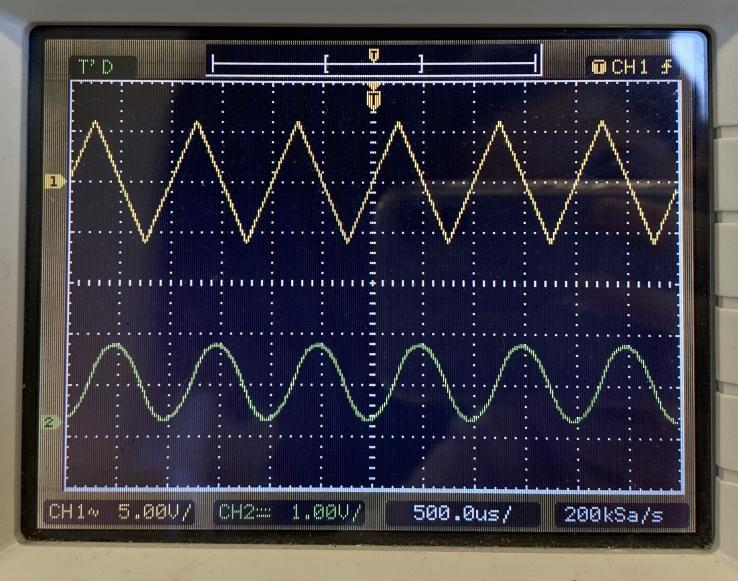
\includegraphics[width=4.5cm]{Dreieck.jpg}
		\caption{Dreiecksspannung}
	\end{subfigure}
	~
	\begin{subfigure}[b]{0.3\textwidth}
		\centering
		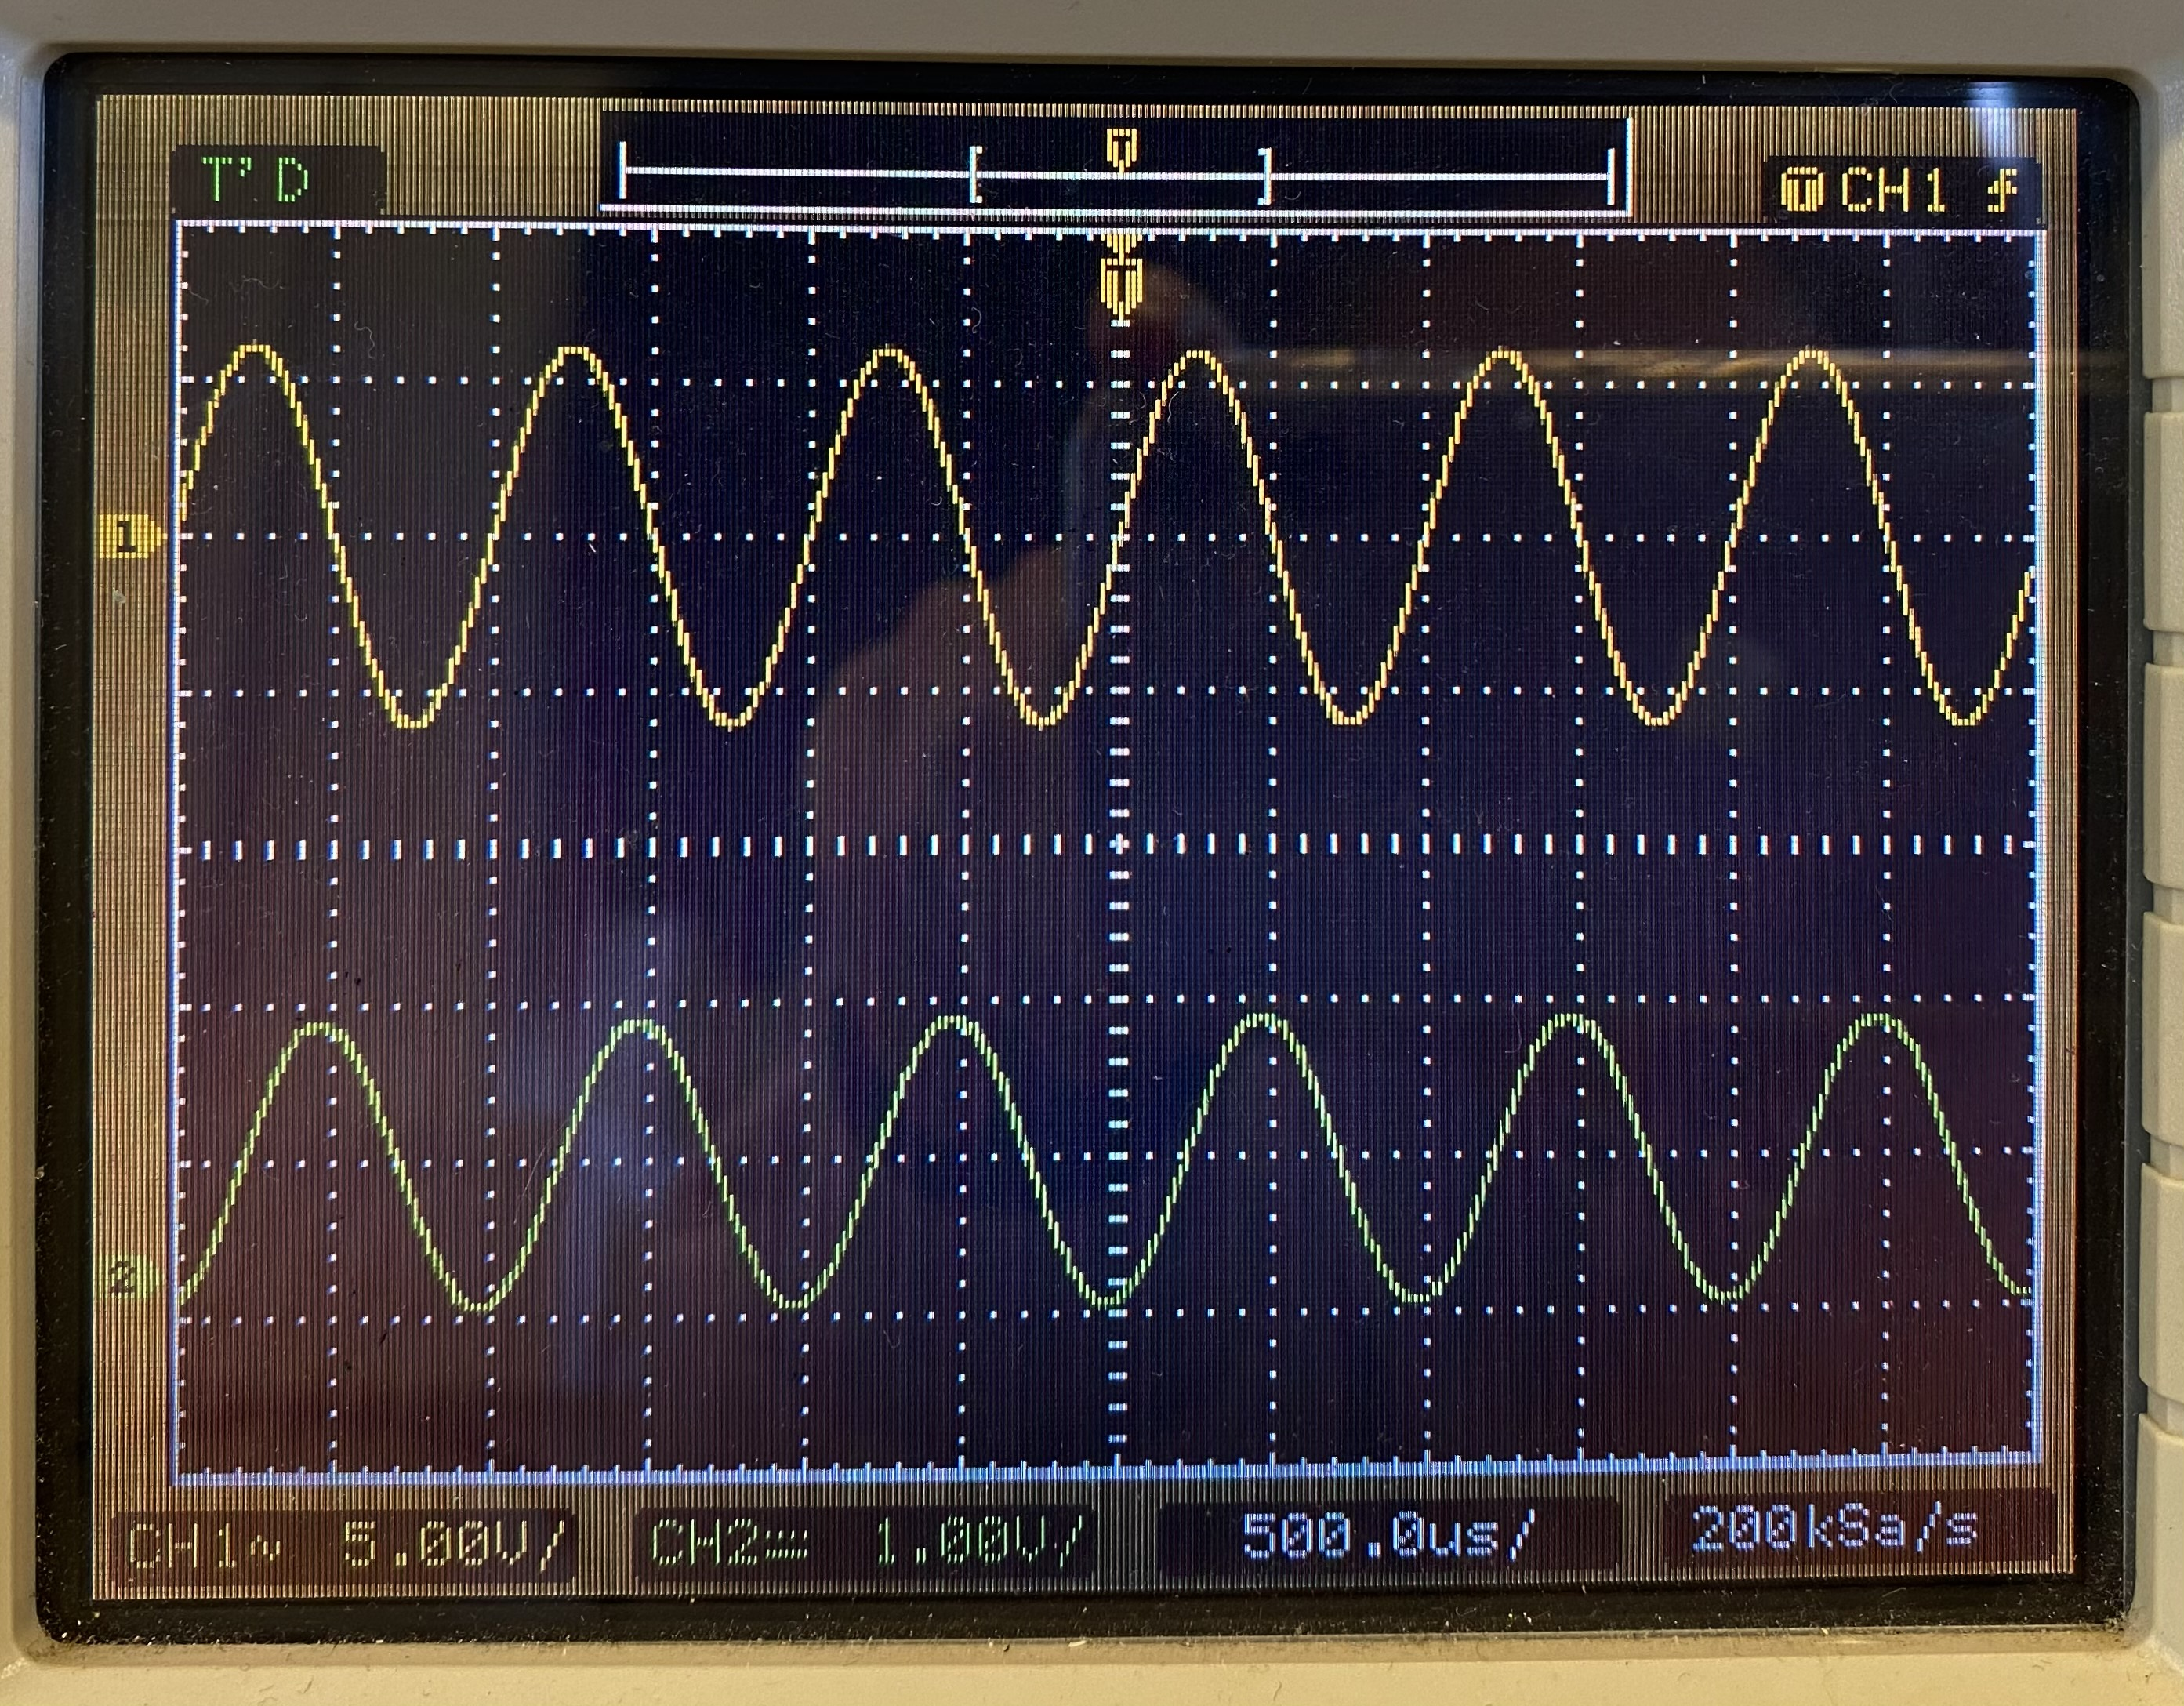
\includegraphics[width=4.5cm]{Sinus.jpg}
		\caption{Sinusspannung}
        \label{fig:sinus}
	\end{subfigure}
    \caption{Fotos vom Oszilloskop}
\end{figure}

\noindent
    Exzeplarisch erklärt sieht man in der letzten Abbildung (\ref{fig:sinus}) die anliegende Sinusspannung. Dazu unten die Kondensatorspannung die als phasenverschobene Sinusspannung gegeben ist.
    Da das Integral von Sinus der Cosinus ist und der Cosinus lediglich ein phasenverschobener Sinus ist, ist zu sehen, dass der RC Kreis unter bestimmten Voraussetzungen als Integrator arbeiten kann.

